\chapter{Introdução}
\label{intro}


A informação pode ser considerada o maior ativo de uma empresa ou corporação no cenário econômico moderno, de acordo com \citeonline{fraimovich2020role}, e este fato destaca que os proprietários devem se preocupar com o resguardo de seus dados, principalmente no que tange à confidencialidade, integridade e à disponibilidade destes. A quarta revolução industrial, ou ``Indústria 4.0'', termo que fora criado pelo Presidente do Fórum Econômico Mundial, \citeonline{schwab2019quarta}, descreve a mudança de paradigma na forma como as pessoas vivem e se relacionam e, em especial, como as empresas e corporações necessitam saber gerir as informações de forma com que sobrevivam num mercado competitivo, reforçando a supracitada necessidade de resguardo dos dados por meio da implementação de métodos de Segurança da Informação. 

A heterogeneidade dos acessos à Internet no que diz repeito ao conteúdo e à anatomia dos pacotes trafegados na rede mundial torna o processo de identificação de ataques (ou de pacotes maliciosos) um problema de pesquisa sobre o qual a comunidade acadêmica tem se dedicado, conforme observar-se-á no decorrer desta dissertação, em especial na Seção \ref{rev_sistematica}. Neste sentido, diversos tipos de IDS têm sido empregados para analisar o ``comportamento da rede'' à fim de detectar fluxos maliciosos que objetivam, necessariamente, causar danos aos ativos, em especial, à informação.

O Objetivo Geral da presente Dissertação de Mestrado é apresentar um modelo de detecção de intrusão utilizando \textit{Ensemble Machine Learning} por meio da técnica de \textit{Stacking}. Trata-se de uma forma de aprendizagem de padrões de ataques realizada por um \textit{committee} (conjunto) de classificadores. Ademais, apresenta-se uma maneira eficaz de seleção de classificadores por meio da Diversidade (\textit{Diversity Pruning}). Os Objetivos Específicos refletem a maneira como buscou-se alcançar o Objetivo Geral bem como a estrutura organizacional da pesquisa:

\begin{itemize}

\item Apresentar Introdução (Capítulo \ref{intro}) ao tema objeto da pesquisa de forma com que sejam justificados os esforços na realização da presente dissertação, bem como realizada a contextualização, apresentados os objetivos geral e específicos e a metodologia empregada;

\item Documentar o estado-da-arte por meio da apresentação de uma Revisão Sistemática da Literatura (Subseção \ref{rev_sistematica}), apresentando ao leitor uma linha do tempo no que tange à evolução do tema pesquisado ao longo dos últimos cinco anos;

\item Extrair as tendências de utilização de classificadores, \textit{datasets}, métodos de \textit{Ensemble} e demais dados relevantes por meio do processamento dos trabalhos relacionados (Subseção \ref{compilacao-rsl});

\item Organizar os resultados obtidos para todos os trabalhos correlatos de forma com que seja possível compará-los (Subseção \ref{compilacao-rsl});

\item Documentar o funcionamento dos Sistemas de Detecção de Intrusão quanto a forma como são dispostos topologicamente nas redes e na forma como manipulam os pacotes (Seção \ref{sec:ids});

\item Apresentar uma visão geral do Processo de \textit{Data Mining} em \textit{datasets} (Seção \ref{sec:datamining}) bem como as bases de Classificação, Regressão e \textit{Clustering} para \textit{Machine Learning} (Seção \ref{sec:machinelearning});

\item Descrever as principais técnicas de \textit{Ensemble Learning} (Seção \ref{Ensemble}) de forma com que seja fundamentada a sua utilização com destaque para o método \textit{Stacking} e para o \textit{Diversity Pruning};

\item Apresentar a modelagem (produto desta dissertação) de um Sistema de Detecção de Intrusão baseado em \textit{Stacking} por \textit{Diversity Pruning}, desde o processo de concepção (Capítulo \ref{cap-metodologia}) até os resultados obtidos (Capítulo \ref{result});

\item Observados os resultados obtidos, apresentar as considerações finais e a conclusão (Capítulo \ref{conclusoes}).


\end{itemize}


A problemática que pautou o desenvolvimento desta Dissertação de Mestrado foi: a seleção de classificadores por meio de \textit{Diversity Pruning} pode fornecer uma estrutura adequada para a composição de \textit{Stackings} que geram incremento de \textit{performance} na detecção de intrusão para dados de redes de computadores?

Justificam os esforços empregados na presente dissertação o crescente número de incidentes de segurança da informação. De acordo com o Centro de Estudos, Respostas e Tratamentos de Incidentes de Segurança da Informação no Brasil  \cite{certbr:online}, tem-se observado uma crescente considerável em relação aos ataques que são notificados à entidade responsável pela tomada de decisões no âmbito em questão no Brasil. A Figura \ref{fig:cert} ilustra esse cenário:

\begin{figure}[H]
\centering
\caption{Estatísticas gerais sobre ataques notificados ao CERT.br por ano.}
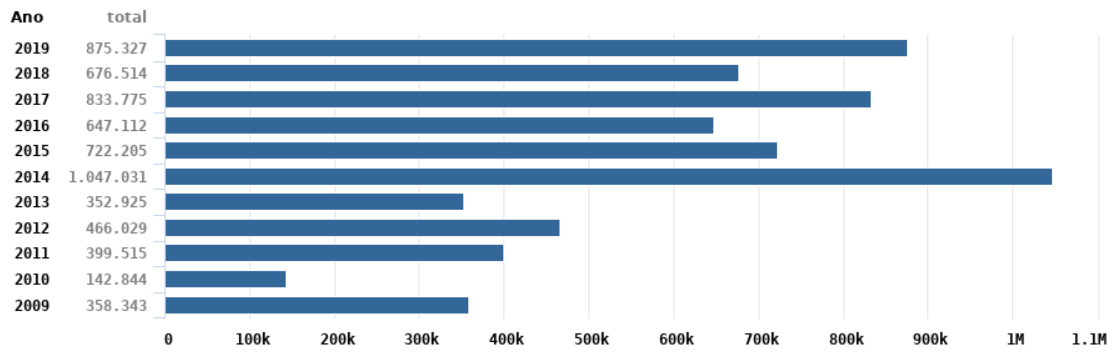
\includegraphics[width=16.3cm,height=\textwidth,keepaspectratio]{figs/incidentes.png}
\newline\centering{Fonte: Adaptado de \citeonline{certbr:online}}\label{fig:cert}
\end{figure}

Independente da variação entre os anos (eixo $y$) é nítido observar na Figura \ref{fig:cert} o crescimento do número de ataques (eixo $x$), o que justifica por parte das empresas ou corporações e até mesmo das academias o emprego de esforços na implementação de IDS e no estudo de formas cada vez mais efetivas de se detectar atividades maliciosas na rede (ou mesmo uma invasão consumada, denominada \textit{infiltration}) em tempo para que se possam tomar decisões de prevenção de intrusão.


A metodologia empregada no processo de criação desta dissertação consistiu no emprego de Revisão Sistemática da Literatura (Seção \ref{rev_sistematica}) extraindo dados relevantes para trabalhos correlatos obtidos por meio de protocolo pré-definido. De acordo com os métodos de pesquisa \cite{gerhardt2009metodos}, o presente trabalho, quanto à abordagem trata-se de pesquisa quantitativa; quanto à natureza trata-se de pesquisa aplicada; quanto aos objetivos trata-se de pesquisa explicativa e, quanto aos procedimentos trata-se tanto de pesquisa experimental. A modelagem do Sistema de Detecção de Intrusão proposto fora realizada utilizando as linguagemns de programação R (pré-processamento) e Python (modelagens e testes) por meio de bibliotecas de \textit{machine learning} e os testes foram executados em seis diferentes \textit{datasets} que compõem o conjunto de dados CICIDS-2017. Mais detalhes acerca dos materiais e métodos podem ser observados no Capítulo \ref{cap-metodologia}.
